
% latex-sample.tex
%
% This LaTeX source file provides a template for a typical research paper.
%

%
% Use the standard article template.
%
\documentclass{article}
\usepackage[affil-it]{authblk}
\usepackage{multirow}
% The geometry package allows for easy page formatting.
\usepackage{geometry}
\geometry{letterpaper}

% Load up special logo commands.
\usepackage{doc}

% Package for formatting URLs.
\usepackage{url}
\usepackage{listings}
\usepackage{color}
\usepackage{minted}
% Packages and definitions for graphics files.
\usepackage{graphicx}
\usepackage{epstopdf}
\DeclareGraphicsRule{.tif}{png}{.png}{`convert #1 `dirname #1`/`basename #1 .tif`.png}

\lstset{frame=tb,
  language=SQL,
  aboveskip=3mm,
  belowskip=3mm,
  showstringspaces=false,
  columns=flexible,
  basicstyle={\small\ttfamily},
  numbers=none,
  numberstyle=\tiny\color{gray},
  keywordstyle=\color{blue},
  commentstyle=\color{dkgreen},
  stringstyle=\color{mauve},
  breaklines=true,
  breakatwhitespace=true,
  tabsize=3
}
%
% Set the title, author, and date.
%
\title{Final Report of "Hadoop YARN Cloud Configuration Tool"}

\author{Group 9: Shiqian Xu, Jiang Gu, Pengyu Li, Liang Dong}
\affil{Course: Data Intensive Computing}
\date{2015-12-07}

%
% The document proper.
%
\begin{document}

% Add the title section.
\maketitle
\newpage
% Add an abstract.
\section{Abstract}
In this project, we deploy Hadoop Cluster on Amazon AWS cloud platform using Apache Ambari, monitor runtime information of the Hadoop eco-system using Ambari metrics, and add user-defined alerts into Ambari. Based on our user-defined alerts which can be generated by Ambari, we set up our monitor process and periodically monitor the user-defined alerts. According to our monitoring data and duration time of each alerts, we design our scale policy. Then we use each alert to trigger our scale process based on the scale policy, and execute the scale process to upscale or downscale. We provide RESTful service and WebUI to ease the deployment of auto-scaling cluster. Thus we put forward a scale solution and strategy of how to scale out Hadoop Cluster and compare the Hadoop Cluster performance of before scale and after scale using different data sets.
	
\section{Introduction}
The report gives a description on how to deploy Hadoop YARN cluster using Apache Ambari, monitor the cluster and later on use the monitoring data to scale the cluster by adding or deleting data nodes based on status of the instance or job type. \textbf{Figure~\ref{fig:architecture}} gives an overview on the whole system looks like.

The report is organized as follows. Section 3 introduces the system architecture. Section 4 mainly talks about the deployment of Hadoop Cluster on EC2. Section 5 gives an overview on the different techniques that we have used to get the monitoring data. Section 6 illustrates the study in answering three questions: why, when and how we should implement scaling out.

The application will integrate Hadoop provisioning and monitoring capabilities with the Ambari Rest API. Monitoring long and complex Hadoop jobs can be challenging as stated by Wadkar and Madhu in ¡°Monitoring Hadoop¡±[\ref{ref:wadkar}]. The Ambari project is aimed at making Hadoop management simpler by developing software for provisioning, managing, and monitoring Apache Hadoop clusters.

The focus of this report is on how to scale the cluster based on the monitoring data. It will mainly talks about why and when we should scale out the Hadoop Cluster. There are two assumptions in our project. The first one is that data intensive jobs are suitable for scaling out. The other is that scaling out is necessary when the job exceeds a certain threshold of YARN memory usage. And we will do experiments on two kinds of jobs(data intensive versus computing intensive) in Hadoop cluster and use various metrics to testify our assumptions.

The goal of our system is to provide Administrator and Hadoop user with a choice of starting a Hadoop cluster without knowing the number of instances before head. The system is able to auto adjust number of instances in the cluster to fit the resources that needed in running different jobs. The design of this system suits for elastically deploy cluster to cope with loads dynamically and is especially useful in today's pay-as-you-go scenarios when users are using a Platform as a Service cloud and don't want to pay for resources that is not being currently needed, but will be able to fast scale out when needed.

%
% Body text.
%
\section{System Architecture}

\begin{figure}[ht!]
 \centering
 \includegraphics[width=0.7\textwidth,natwidth=700,natheight=600]{architecture.png}
 \caption{Architecture of Hadoop project}
 \label{fig:architecture}
 \end{figure}
 
This is our system architecture which mainly includes three parts. The first part is the Hadoop Yarn Cluster, we deployed our Hadoop Cluster on Amazon AWS using EC2 instances. The cluster includes Resource manager, Node manager, Data nodes and Name nodes. The second part is the Ambari. In this part, we use Apache Ambari to monitor our Hadoop Cluster, which is a framework for deploying, managing and monitoring Hadoop Cluster, and provides plenty of Restful APIs and tools to simplify the operations of Hadoop Clusters. We use Apache Ambari to deploy and monitor our Hadoop Cluster. In this part, we have defined our own alerts(Allocated memory alert and Running application alert), and added these self-defined alerts into Ambari Server using REST APIs. The third part is the scale module, which includes alerts component, monitor component, scale component, Web UI and Command Line Interface. In the third part, we have designed several REST APIS to add cluster, instance and policy into the Hadoop Cluster. Then we develop our own monitor to monitor the self-defined alerts and design our scale policy to do the scaling. Based on monitoring alerts data, our application will execute the scale process(scale out and scale down) according to different scaling policy. which will be monitored by our 

The main jobs of our project are to deploy Hadoop Yarn Cluster on Amazon EC2, monitor the health of Hadoop Yarn Cluster using Ambari metrics and scale out Hadoop Cluster based on our monitoring data. In our scale module, we have defined our own alerts which are used to trigger our scale process. Scale includes scale out process and scale down process. For scale out process, it will be triggered by the allocated memory alert, which will be generated if Hadoop Cluster memory usage is over one threshold. For scale down process, it will be triggered by the running application alert, which is generated if running jobs in Hadoop Cluster decrease to the lowest threshold.

\section{Deploy Hadoop YARN Cluster}
In our project, the main job is to deploy, monitor and scale out the Hadoop cluster based on our computing model. Currently, there are several approaches to deploy Hadoop clusters on Cloud, such as following Apache Hadoop Setting up instruction, or using third party tools.

After comparing different methods, We want to adopt Apache Ambari and docker images to deploy the Hadoop clusters on cloud platform. Since Apache Ambari is a completely open operational framework for provisioning, managing and monitoring Apache Hadoop clusters. It includes an intuitive collection of operator tools and a set of APIs that mask the complexity of Hadoop, simplifying the operation of clusters. Docker images are typically very small, which facilitates rapid delivery and reduces the time to deploy new application containers. They also brings in an API for container management, an image format and a possibility to use a remote registry for sharing containers.

These tools and APIs of Apache Ambari and Docker can help us deploy and monitor Hadoop cluster easily. Then we can use these collected data to build our model and scale out the Hadoop cluster.

\subsection{Deployment Steps}
Apache Ambari includes Ambari Server and Ambari Agent. We deployed Ambari Server and Agents on AWS EC2 since cloud computing resources are cheap and convenient. The deployment process includes the following steps. The deployment result is shown in \textbf{Figure~\ref{fig:deploymentResult}}. \\
(1)Create EC2 instances on AWS and setup Ambari Environment\\
(2)Setup Ambari Server and Agents on EC2 using docker images\\
(3)Setup consul on EC2 as an Ambari DNS server\\
(4)Deploy Hadoop Cluster using Ambari\\
(5)Test Hadoop Cluster\\
\begin{figure}[ht!]
 \centering
 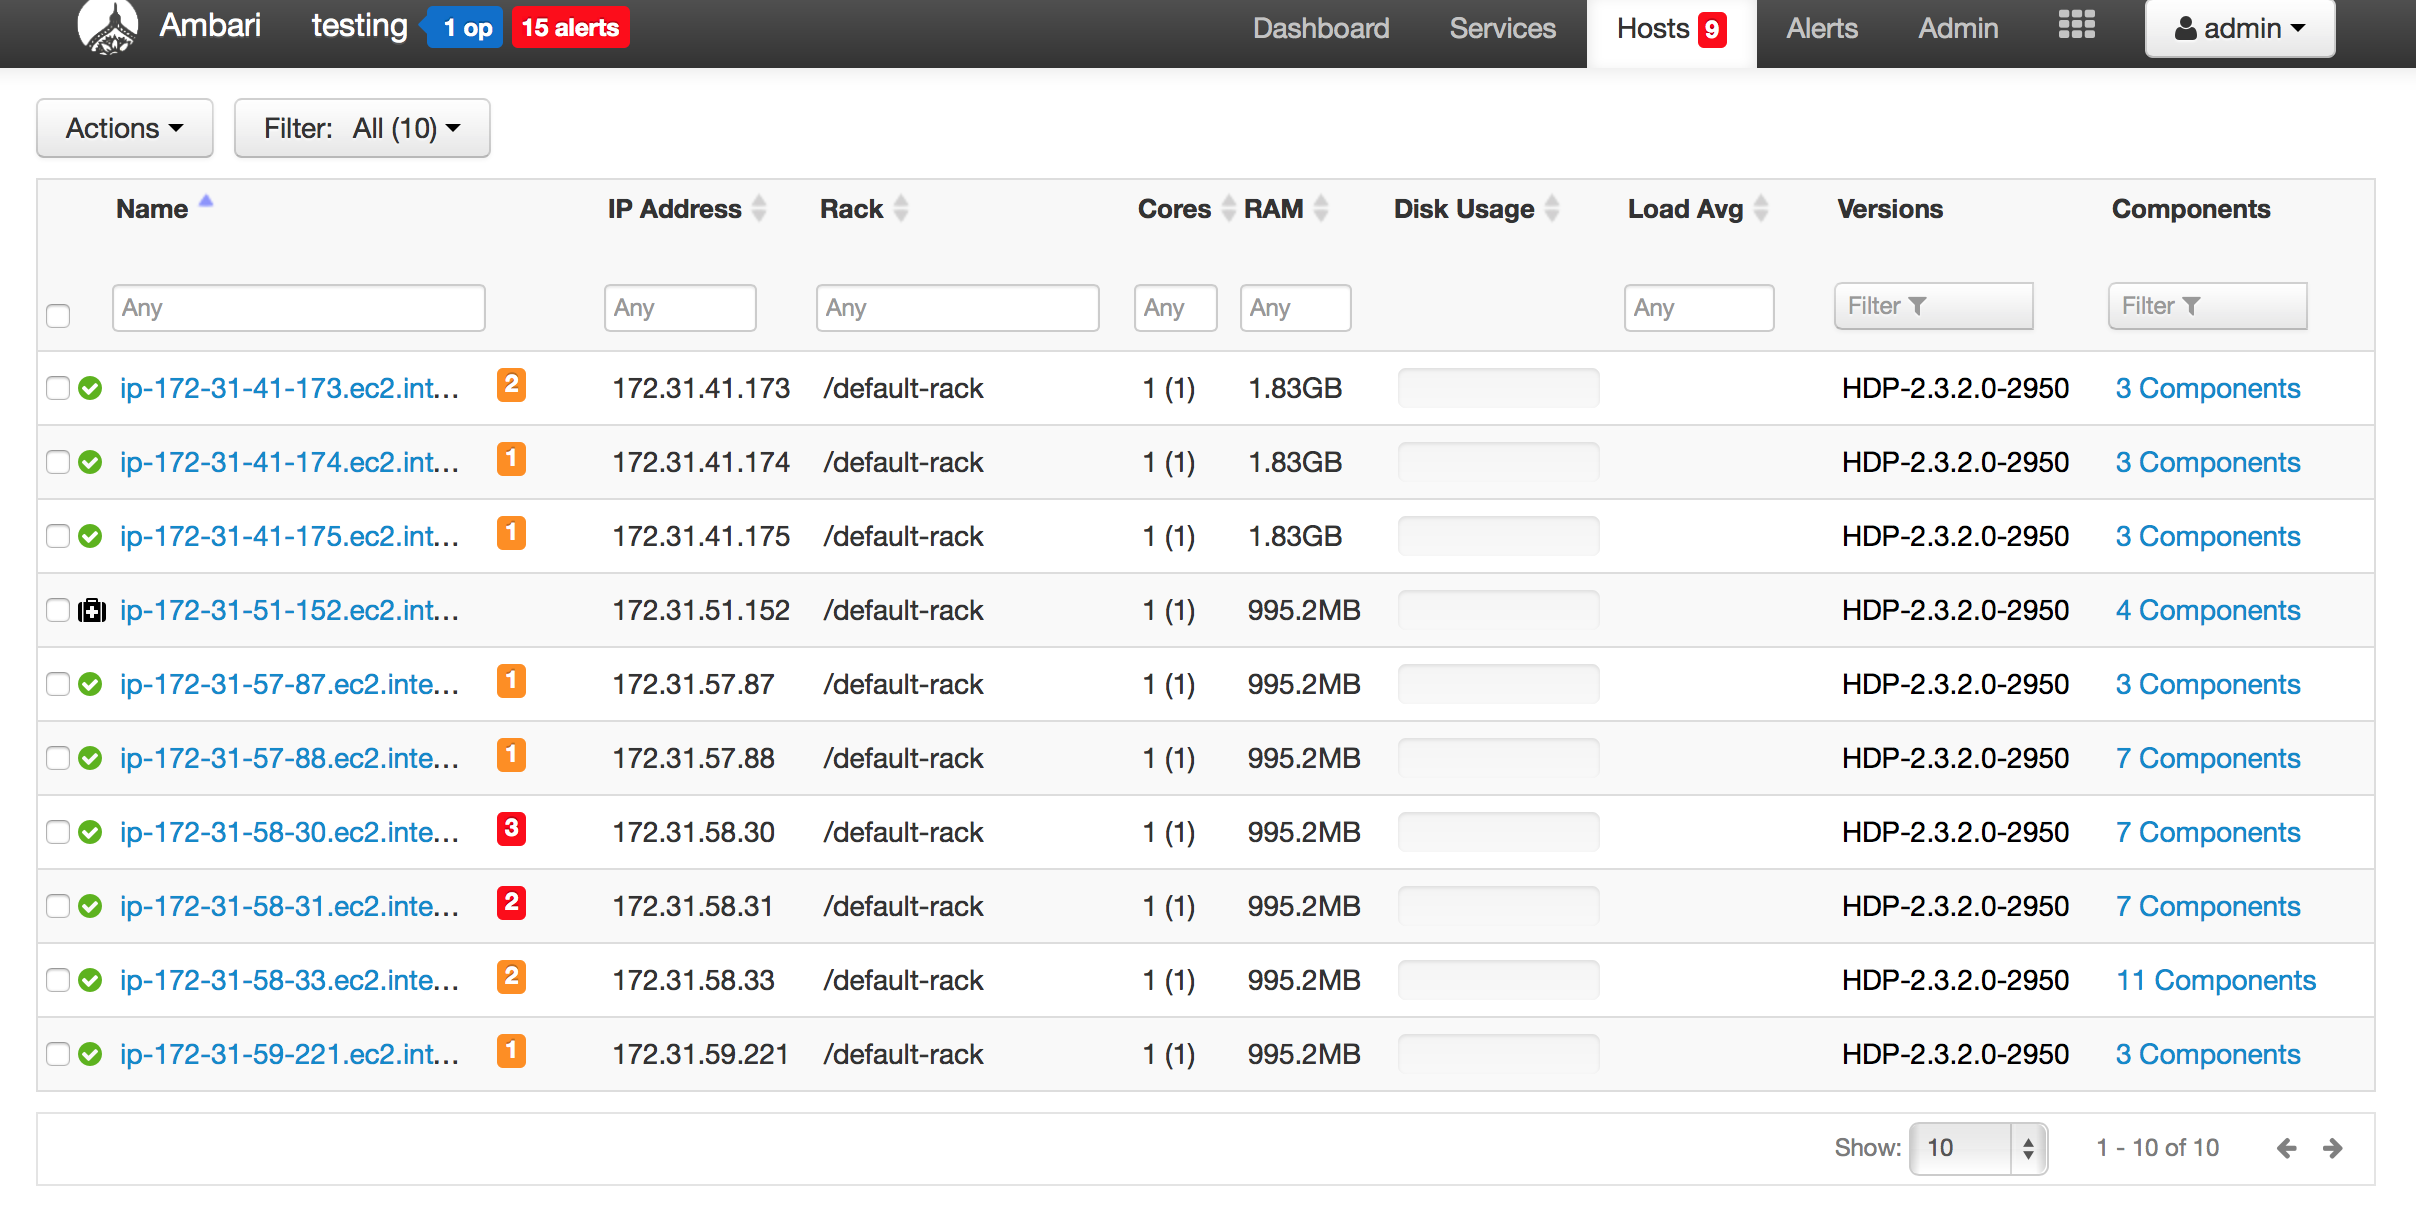
\includegraphics[width=0.7\textwidth,natwidth=1200,natheight=400]{deployment.png}
 \caption{Deployment Result}
  \label{fig:deploymentResult}
 \end{figure}

\subsection{Deployment Problem}
During our deployment process, we encountered a problem that our Ambari Server cannot communicate with Ambari Agents. Thus, the server cannot execute the Hadoop cluster deployment commands.
\subsection{Solution to Deployment problem}
In order to figure out this problem, we analyzed the both log files of Ambari Server and Agents, and found that our Ambari Server cannot identify the hostname of Ambari Agents. For this problem, we tried two solutions.

The first solution is to register each agent¡¯s IP address and hostname to Agent Server. The advantage is that it can help Ambari Server communicate with Agents. But the disadvantages of this solution are obvious, 1) The register process is complex. Since all agents need register to Ambari Server, and Ambari Server need execute shell scripts and add Agent's¡¯ IP address and hostname into Server. 2) If Ambari Server is gone, the whole system will crush. When setting up a new Ambari Server, all agents need register again.

The second solution is to set up a DNS server for all Ambari Server and Agents. Here we adopt Consul to provide DNS server, which is a tool for discovering and configuring services in your infrastructure. The advantages of this solution are, 1) All Ambari Server and Agents need register to Consul once. 2) If a new Ambari Server is setup, it just needs get all Agents¡¯ information from Consul. 3) It can increase the system¡¯s robustness and availability.

After comparing above two solutions, we adopted the second one to solve the problem, and this method can implement our solution pretty well.




\section{Monitor Hadoop YARN Cluster}
In order to scale the Hadoop YARN cluster, we should first decide whether it is necessary to scale out a cluster.  However, without monitoring data, the scale is misleading. Therefore, the first step we should take is to get the runtime information of the Hadoop eco-system. \textbf{Figure~\ref{fig:monitorStructure}} is the infrastructure that we have utilized to achieve monitoring module which served as the key decision for scaling feature.

\begin{figure}[ht!]
 \centering
 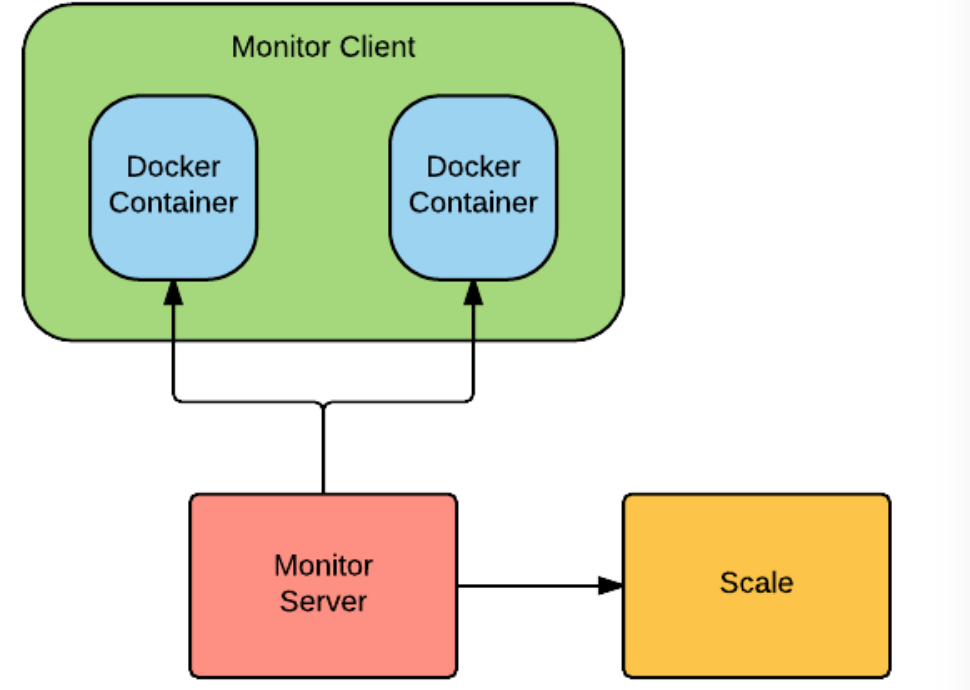
\includegraphics[width=0.6\textwidth,natwidth=500,natheight=300]{fig2.png}
 \caption{Monitor Structure}
 \label{fig:monitorStructure}
 \end{figure}

There are several ways that we can implement the infrastructure, such as through the Ambari Dashboard, the Amazon EC2 Monitoring Dashboard and implementing our own monitoring infrastructure such as Elasticsearch, Logstash and Kibana. We will then look into the data we get from Ambari Monitor Dashboard and EC2 metrics and decide whether we need more information in order to build a more applicable scaling strategy model for scaling cluster to improve the performance of MapReduce2 Job.
\subsection{Ambari Dashboard}
From Ambari Dashboard, we can get most information of the Hadoop system, HDFS status along with many Hadoop services such as ZooKeeper. We can add more widgets to the main dashboard to log more information and get the data from the widgets UI. We have run a sample Hadoop Job to get more understanding of how the monitoring data will look like.
\subsubsection{HDFS Monitoring Metrics}
For HDFS, the metrics are able to provide with the following data, shown in \textbf{Table~\ref{table:hdfsMetrics}}. We can easily tell from the metrics that how much percentage disk is utilized by the DFS or System, which will contribute to the build of the scaling strategy model.
\begin{table}[ht!]
\begin{center}
\begin{tabular}{ |c|c|c| }
\hline
NameNode & Started \\
\hline
SnameNode & Started \\
\hline
DataNodes & 1/1 Started \\
\hline
DataNodes Status & 1 live / 0 dead / 0 decommissioning \\
\hline
NameNode Uptime & 1.01 hours\\
\hline
NameNode Heap & 203.1 MB / 998.4 MB (20.3\% used)\\
\hline
Disk Usage (DFS Used) & 1.4 MB / 6.7 GB (0.02\%)\\
\hline
Disk Usage (Non DFS Used) & 4.9 GB / 6.7 GB (71.99\%)\\
\hline
Disk Usage (Remaining) & 1.9 GB / 6.7 GB (27.99\%)\\
\hline
Blocks(total) & 24\\
\hline
Block Errors & 0 corrupt / 0 missing / 24 under replicated\\
\hline
Total Files + Directories & 56 \\
\hline
Upgrade Status & No pending upgrade\\
\hline
Safe Mode Status & Not in safe mode\\
\hline


\end{tabular}
\end{center}
\caption{HDFS Monitor Metrics}
\label{table:hdfsMetrics}
\end{table}

\subsubsection{YARN Monitor Metrics}
For YARN Monitor, we are able to get the following data as the \textbf{Table \ref{table:yarnMetrics}} shows. We will have the Resource Manager Heap size and how many applications are currently submitted which are pending or running. The cluster memory information will also give us a hint whether to perform a scale.
\begin{table}[ht!]
\begin{center}
\begin{tabular}{ |c|c|c| }
\hline
ResourceManager Heap & 16.8MB/989.9MB(1.7\% used) \\
\hline
Containers & 0 allocated/0 pending/0 reserved \\
\hline
Applications & {3 submitted/0 running/0 pending/3 completed/0 killed/0 failed}\\
\hline
Cluster Memory & {0 Bytes used/0 Bytes reserved/512.0 MB available}\\
\hline
\end{tabular}
\end{center}
\caption{YARN Monitor Metrics}
\label{table:yarnMetrics}
\end{table}

 Other than that, it also has the ability to monitor the CPU utilization of the instance as well as memory utilization and up-time information. \textbf{Figure~\ref{fig:ambariDashboard}} gives a brief snapshot of all the monitor data that we can get from the Ambari side.
\begin{figure}[ht!]
 \centering
  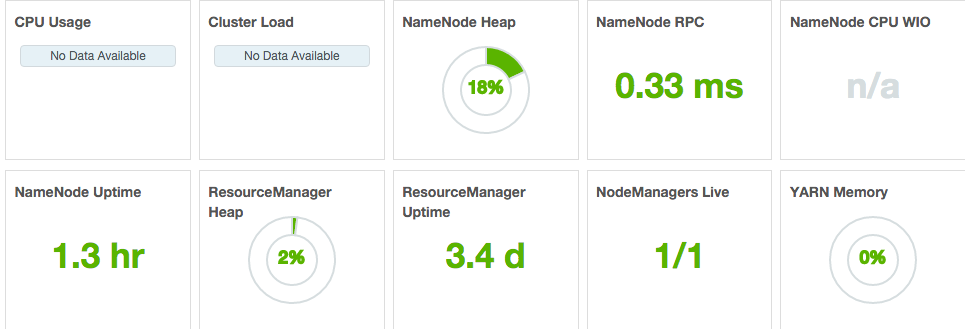
\includegraphics[width=0.8\textwidth,natwidth=1000,natheight=400]{fig4_2.png}
 \caption{Ambari Dashboard}
 \label{fig:ambariDashboard}
 \end{figure}
 \subsection{Amazon EC2 Dashboard}
 Other than Ambari Dashboard, which will give us more information about the Hadoop ecosystem. The monitoring metrics on EC2 will only provide with basic information on Instance level. It knows nothing about what is running on the instance. \textbf{Figure~\ref{fig:aws}} gives us an illusion about the Monitoring metrics on Amazon. As we can see, the data is much less than Ambari provide us. However, the instance level information may also be useful to us, such as the network in/out, as it will give a hint about the network flow of the job which will help us to understand better how Data Intensive Computing works and know if the bandwidth of the network has something to do with our job performance.
\begin{figure}[ht!]
 \centering
  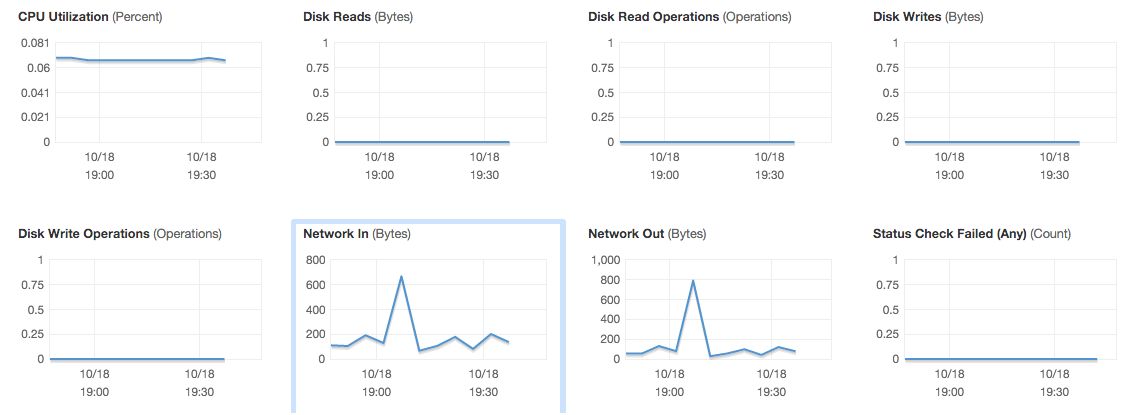
\includegraphics[width=0.8\textwidth,natwidth=1100,natheight=400]{fig4_3.png}
 \caption{Amazon EC2 Dashboard}
 \label{fig:aws}
 \end{figure}

 \subsection{ELK}
 Elasticsearch, logstash combined with Kibana as a monitoring infrastructure is utilized by industry in recent years. No only we can get lots of logs from the system, we can also use it to monitoring our cluster to get some customized information which has not been provided by either Ambari or Amazon EC2. Since we are still not sure what kind of monitoring data will be used to build a scale strategy, no logs has been configured in the system to forward to ELK system. However, we think it is better to get started with the infrastructure in case we may need it later. \textbf{Figure \ref{fig:kibana}} shows how data in Kibana Dashboard is visualized and \textbf{Figure \ref{fig:kibanaFunc}} gives all the alternatives for data manipulation in Kibana can be achieved and visualized.
\begin{figure}[ht!]
 \centering
  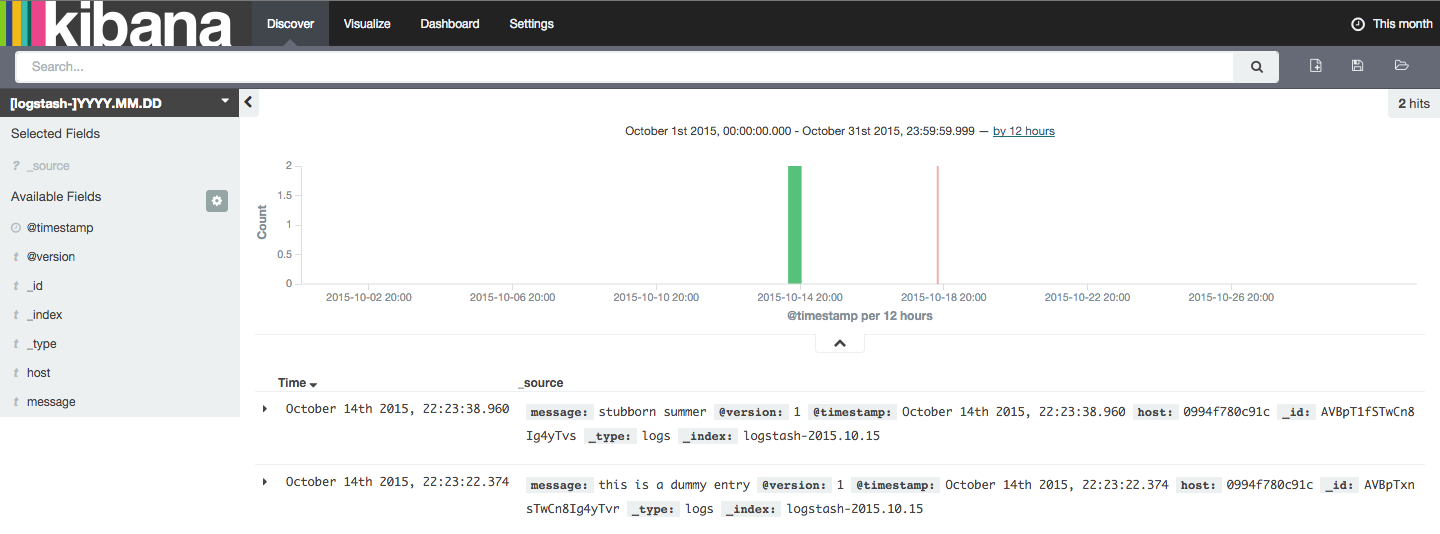
\includegraphics[width=0.9\textwidth,natwidth=1400,natheight=600]{fig4_4.png}
 \caption{Kibana Dashboard}
 \label{fig:kibana}
 \end{figure}
 

\begin{figure}[ht!]
 \centering
  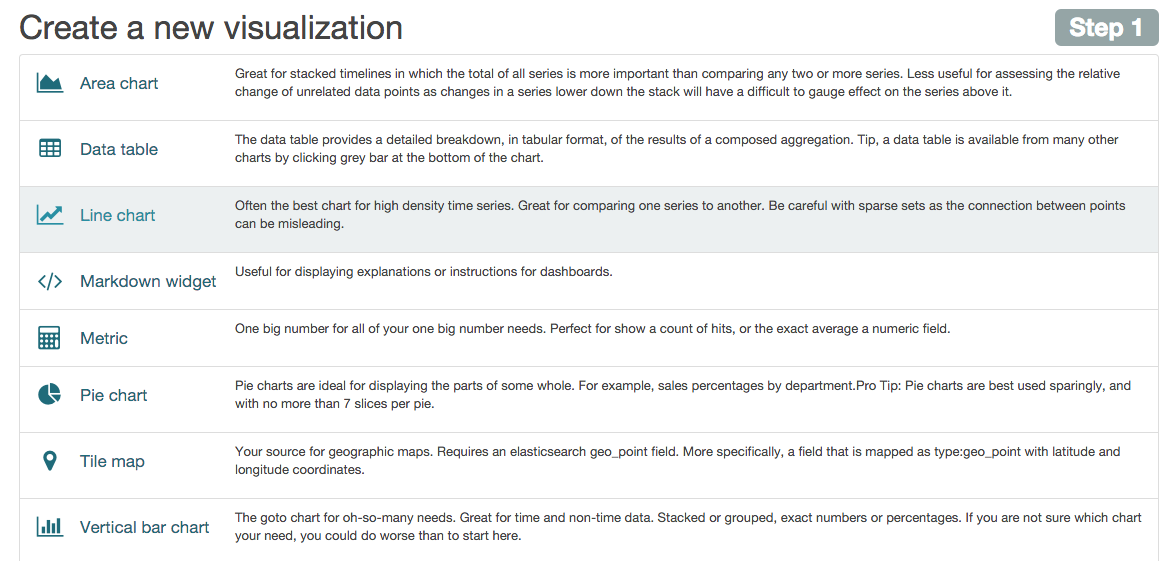
\includegraphics[width=0.9\textwidth,natwidth=1200,natheight=400]{fig4_5.png}
 \caption{Kibana function}
 \label{fig:kibanaFunc}
 \end{figure}
 \subsection{Conclusion}
 We believe the above three kinds of monitoring process will provide with sufficient data to build our scaling model according to different kinds of datasets and jobs. Therefore, less efforts will be spent on this section, we will be focusing more on scale part such as figuring the data set which can be used and how to make the scale actually works.
 
\section{ Auto Scale out Hadoop YARN Cluster}
We consider the cluster used in above experiment is static because the hardware resources are already given when the job is running. We manually modify the cluster size to compare the performance of running jobs. It leads to a question naturally about how to make the cluster itself decide add or remove on the fly. Thus the cluster¡¯s throughput can be increased or decreased based on the cluster load and scheduled applications to achieve better performance without stopping the cluster.	

The key point here is to solve when to make an adjustment. Since we observed that the performance did vary when cluster size changed, the cluster adjustment should based on the real-time performance metrics. These metrics could be collected and queried by via elastic-search. The YARN allocate resource based on memory, a simple schema is to ensure a stable memory usage of the cluster. This means when a memory usage exceed a maximum value, the cluster choose to add node or to remove when a low memory usage. The schema might make little difference to a single running job, but it is meaningful when multiple jobs submitted to the cluster. The process includes complicated balance of both HDFS data and YARN resource when cluster changed. We are still actively working on it. If the stable memory policy works, we can also apply similar policy like stable performance or stable cost to the auto-scale schema.
% * <jesse.xu.20@gmail.com> 2015-12-08T04:15:22.181Z:
%
% ^.
% * <jesse.xu.20@gmail.com> 2015-12-08T04:15:19.922Z:
%
% ^.
\subsection{A small detour}
We first implemented our own monitor system. The system in written design and Java, which utilized the Ambari API[\ref{ref:ambariAPI}] and did a sliding average to check on memory and disk information. When abnormality is detected, it will trigger a scaling event and our handler will take over to perform a scale. However, later on when we kept digging the Ambari API, we found out that its server provided a service called \textbf{alert}, which would throw out an alert when some conditions were met. Therefore, instead of implementing our own monitor system for every module we care about, we could only implement a monitor on its alert system and monitor if there exists an alive alert on that module and the status of the alert.
\subsection{Ambari Alert}
In the project, we have utilized Apache Ambari to deploy and monitor our Hadoop Cluster. Ambari use Ambari Metrics to monitor the health of Hadoop Cluster, it can monitor plenty of health data relevant to Hadoop Cluster. We can see them from below diagram. 
\begin{figure}[ht!]
\centering
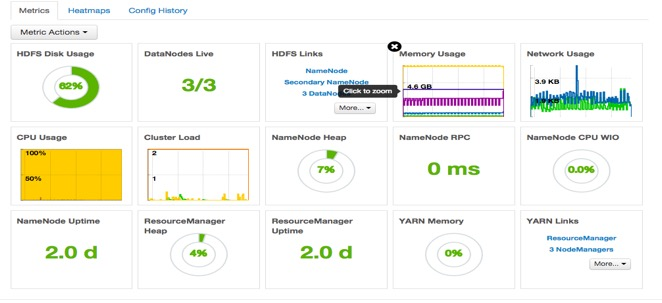
\includegraphics[width=0.8\textwidth,natwidth=1000,natheight=800]{AmbariMetrics.png}
\caption{Ambari Metrics}
\label{fig:AmbariMetrics}
\end{figure}
From Figure~\ref{fig:AmbariMetrics} diagram, we can get lots of monitoring data, such as Disk Usage, Memory Usage, Network Usage and CPU Usage. Based on these monitoring data, Ambari can generate kinds of useful alerts. For example, Figure~\ref{fig:AmbariAlerts} diagram shows different alerts provided by Ambari. 
\begin{figure}[ht!]
\centering
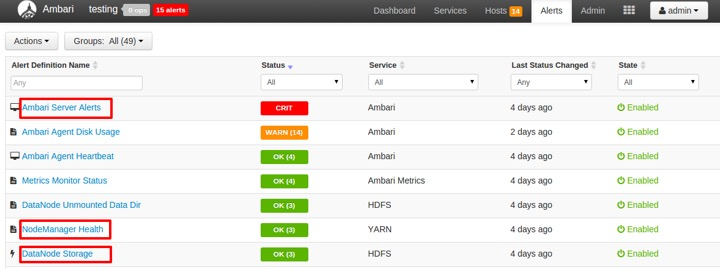
\includegraphics[width=0.8\textwidth,natwidth=1000,natheight=800]{AmbariAlerts.png}
\caption{Ambari Alert}
\label{fig:AmbariAlerts}
\end{figure}
According to Figure~\ref{fig:AmbariAlerts} alert diagram, we can see NodeManager Health alert, DataNode Storage alert and etc. These alerts include the attributes of status, relevant service, duration time and state. The goal of our project is to automatically scale up or down Hadoop Cluster. 
Our scale solution is based on Ambari Alerts. That’s because Ambari provides enriched monitoring data and user customized alerts. 
In our scale solution, we have defined our-own alerts, which are Allocated memory alert and Running application alert. 
\begin{figure}[ht!]
\centering
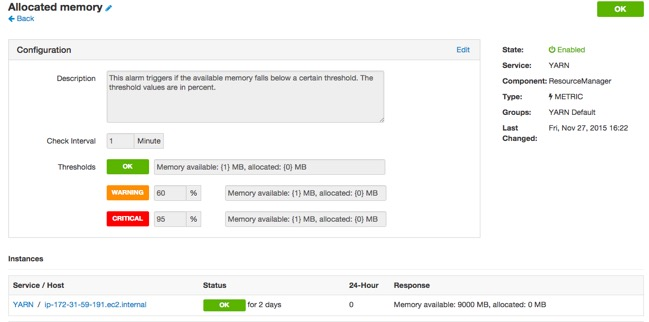
\includegraphics[width=0.8\textwidth,natwidth=1000,natheight=800]{AllocatedMemoryAlert.png}
\caption{Allocated Memory Alert}
\label{fig:AllocatedMemoryAlert}
\end{figure}
From Figure~\ref{fig:AllocatedMemoryAlert} our-own Allocated memory alert, we defined the attributes of check interval and thresholds values. The checkpoint interval is the frequency of alert checking the monitoring data. We also can define different thresholds values, such as when memory usage is lower than 60\%, Ambari will generate an \textbf{OK} alert, and when memory usage is over 60\% and lower than 95\%, Ambari will generate a \textbf{Warning} alert, and when memory usage is over 95\%, Ambari will generate a \textbf{Critical} alert. In each alert, it still has a duration time which means that how long the alert lasts. Based on above thresholds value and duration time, we can make our scale policy. Meanwhile, we use Ambari alert to trigger our scale process. 

\subsection{Alert-based Scaling System(AbSS)}
After understanding the Ambari alert system, we put forwarded the following system, an Alert-based Scaling System, as shown in \textbf{Figure~\ref{fig:scaleProcess}}. In order to use our service, you will need to first add alert definitions to our system and then work out a policy with us on how you would like your cluster to be scaled when that alert is triggered. After that, you should register your AWS instances to our persistent database, instance pool in Figure~\ref{fig:scaleProcess}, so that we could use them during the scaling up/down process.\\
Our service will check with Ambari server every 10 seconds to see if there is a new alert triggered which is registered with our service. If a specific alert is detected and it meets the requirement set in our policy, our system will publish a scaling event, either marked us downscale or upscale and the nodes to be deleted/added to our scaling events pool. The event handler will then go ahead to handle all the event handler. The producer-consumer model enables asynchronism, which breaks the dependency between the producer and the consumer, which can add a lot of performance improvement in our system, shown in \textbf{Figure~\ref{fig:systemWorkflow}}.

\begin{figure}[ht!]
\centering
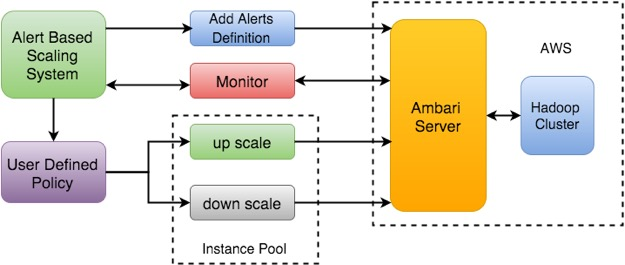
\includegraphics[width=0.8\textwidth,natwidth=1000,natheight=800]{scalingProcess.png}
\caption{Scaling Process}
\label{fig:scaleProcess}
\end{figure}
 
\begin{figure}[ht!]
 \centering
  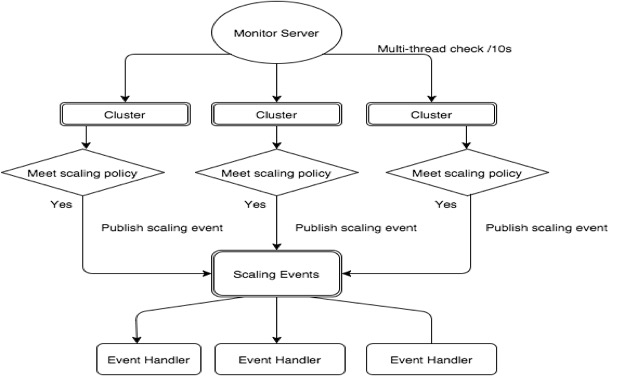
\includegraphics[width=0.8\textwidth,natwidth=1000,natheight=800]{systemWorkFlow.png}
 \caption{Scaling System Work Flow}
 \label{fig:systemWorkflow}
 \end{figure}
The scaling process including starting new instance, installing the components and adding into cluster. The process of preparing new instances takes up to 20 minutes. Considering the scaling system should respond quickly to a scaling event, we bootstrap the initialization of instances by pre-install related components (HDFS NAMENODE and YARN resource manager by default) and make these instances standby in instance pool. The instance pool is maintained in an SQL database, see detailed database schema in the Appendix.  Thus, new instances could be added and join the cluster service in 1-3 minutes, which makes difference to running applications and cluster workload. In the down scale phase, the instances are rejected from cluster but all components are remained. Data of HDFS are transferred to active nodes. The instances are stopped to save AWS cost but could be waken up easily when upscale event was triggered. 

\subsection{REST Service and WebUI}
We implemented a RESTful service based on JAVA Spring boot. via REST API, we could add monitoring clusters, scaling policy and initialized instances for scaling. We also developed a Web interface for this system based on REST API to simplify the procedure for user to add policy to our system. With UI, it would be even quicker for a user to use with our system to deploy an auto-scaling Hadoop cluster. 
\begin{figure}[ht!]
\centering
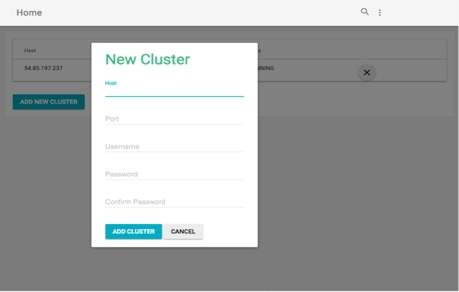
\includegraphics[width=0.5\textwidth,natwidth=1000,natheight=800]{addNewCluster.png}
\caption{Add New Cluster}
\label{fig:addNewCluster}
\end{figure}
\begin{enumerate}
  \item Register Cluster with \textbf{AbSS}(shown in Figure~\ref{fig:addNewCluster})\\
  
  POST /clusters 
  
  GET  /clusters  

  GET  /clusters/\{cluster\_id\} \\
  
  During registration, you will need to provide us with Ambari Information and credentials of your cluster, such as username, password, URL and port information.

\begin{figure}[ht!]
\centering
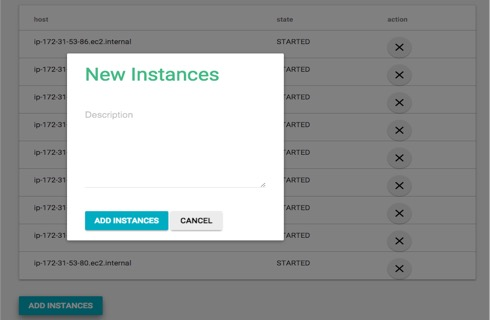
\includegraphics[width=0.5\textwidth,natwidth=1000,natheight=800]{addNewInstance.png}
\caption{Add New Instance}
\label{fig:addNewInstance}
\end{figure}
  \item Add instances to the Cluster(shown in Figure~\ref{fig:addNewInstance})\\
  POST  /clusters/\{cluster\_id\}/instances \\
  GET  /clusters/\{cluster\_id\}/instances \\
  GET  /clusters/\{cluster\_id\}/instances/\{instances\_id\}\\
  
  By adding instances to our cluster, you will need to install the Apache Ambari client and input the private DNS name of your instance.

 
  \item Define scaling policy(shown in Figure~\ref{fig:addNewPolicy})
  
  POST  /clusters/\{cluster\_id\}/alerts/metrics \\
  GET  /clusters/\{cluster\_id\}/alerts/metrics \\
   GET  /clusters/\{cluster\_id\}/alerts/metrics/\{alert\_id\} \\
   
  \begin{itemize}
  \item Choose an alert to monitor and based on that to trigger the scaling
  \item Choose the time to monitor that alert
  \item Choose the alert trigger status(OK, WARNING, CRITICAL)
  \item Choose scale type(Scale up/ Scale down)
  \end{itemize}
 \begin{figure}[ht!]
 \centering
 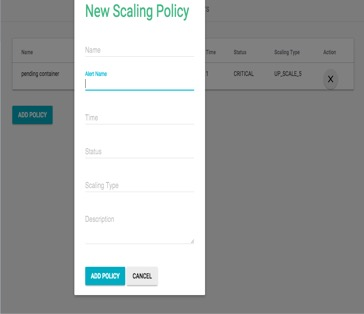
\includegraphics[width=0.4\textwidth,natwidth=1000,natheight=800]{addNewPolicy.png}
 \caption{Define New Scaling Policy}
 \label{fig:addNewPolicy}
 \end{figure}
 
\end{enumerate}


\section{Case Study}
We did two case studies to testify our scaling design and implementation. The first one is auto scaling out the cluster when there is no enough Yarn memory. The second one is to auto scaling out the cluster when there is no pending jobs and no Yarn memory usage. 

The basic assumption of our case studies is that data intensive jobs are suitable for scaling out. Our choices about experiment jobs, metrics and clusters are described as following.\\
\textbf{Jobs}: Computing intensive jobs(like Pi estimate example) versus data intensive jobs(like word count example, tera-sort example, log processing example)\\
\textbf{Metrics}: performance, performance per node,  performance per dollar: derive performance per dollar by dividing raw performance by the capital/acquisition cost of the hardware, CPU usage, YARN memory usage, I/O operation, network overhead. The metrics are already described  monitoring subsection.\\
\textbf{Clusters}: The initial cluster starts from 6 nodes. Each instance type is t2.micro equipped with 1G RAM and single CPU. Then scale out to 9 ,12 nodes of the cluster.

We divide the problem of scaling out the YARN cluster into three sub problems. The first problem is why we need to scale out. We expect scaling out could improve the performance of the cluster and make efficient use of resources. Since AWS charges for the usage of EC2, we should control the cluster at a reasonable size for the trade-off between cost and performance. We need to find a method to calculate the cost and design experiment to test performance.The second problem is when we should scale out the cluster. For this problem, we should add slave nodes in the cluster as the data set becomes larger, and figure out how many slave nodes we should need adjust. In order to solve this problem, we will run different data sets and monitor the Hadoop Cluster, AWS EC2 performance and other related information. Then, based on these information, we will create our data model and give the results of when to deploy and how many data nodes should be adjusted.The third problem is how we scale out the Hadoop Cluster. For this part, our current solution is to develop a scale-out server listening to the running cluster. When an adjustment event was fired, the server should be able to respond by add new nodes to the cluster or remove nodes from the cluster.
 
For the case study of auto scaling out, the initial state of our cluster is one name node and three data nodes. The job is to calculate pi based on quasi-Monte Carlo method. We choose this job because we can add or remove computing demand by setting the number of maps and other parameters The number of maps is set to be 100. And the number of points to be generated is set to  ten million. The scaling policy is that when Yarn memory usage exceeds 60\% for one minute, it will trigger the system to add two nodes in the cluster. In practice, several minutes after the job started, the usage of Yarn memory will reach 85\%, shown in \textbf{Figure~\ref{fig:autoscalingout}}. Then it would trigger the alert,  our system gets the alert and executes the scaling out policy, that means adding 2 data nodes in this case. 
 \begin{figure}[ht!]
 \centering
 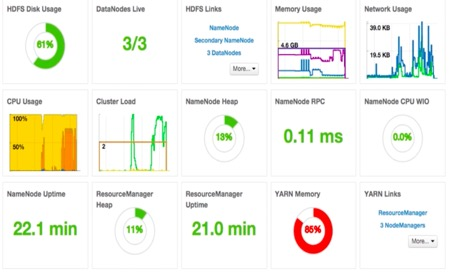
\includegraphics[width=0.8\textwidth,natwidth=1000,natheight=800]{caseScaleOut.png}
 \caption{Case Study of Auto Scaling Out}
 \label{fig:autoscalingout}
 \end{figure}
 
For the case study of auto scaling down, the cluster had 12 data nodes at first, as shown in \textbf{Figure~\ref{fig:autoscalingdown}}. The scaling policy is to remove two data nodes from the cluster when there is no pending jobs and no memory usage for one minute. Then, the cluster is downscaled to the minimum size after several minutes.In practice, you can define both the alerts and scaling policies, like defining how long it takes to trigger the alert.
\begin{figure}[ht!]
 \centering
 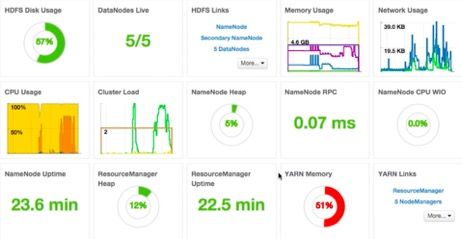
\includegraphics[width=0.8\textwidth,natwidth=1000,natheight=800]{caseScaleDown.png}
 \caption{Case Study of Auto Scaling Down}
 \label{fig:autoscalingdown}
 \end{figure}
 
 \section{Comparison}
 \subsection{Comparison in two clusters}
In order to compare the performance of our auto-scaling solution, we have run the same job (yarn jar hadoop-mapreduce-examples-2.7.1.2.3.2.0-2950.jar pi 100 1000000000) on two clusters, one is auto scaling cluster, the other is no scaling cluster. In auto scaling cluster, job finished in 437.635 seconds, and the no scale cluster need 625.257 seconds to finish the same job. The performance has been improved by 31\%. 

We get the information of containers from Hadoop metrics.
The starting time and duration of containers in the cluster under scaling and no-scaling are shown in \textbf{Figure~\ref{fig:scaling_pi}} and \textbf{Figure~\ref{fig:no_scaling_pi}}. The starting time is shown in X-axis, the length of line represents the duration of each container. From those two graphs, we knew that Auto-Scaling will increase the performance by reducing the total running time. Furthermore, segments are more densely populated in the up right of \textbf{Figure~\ref{fig:scaling_pi}}, showing that the cluster has scaled out and assigned more containers at the same period of time as there are more resources added to the cluster, thus cutting the total running time of the job.
\begin{figure}[ht!]
 \centering
 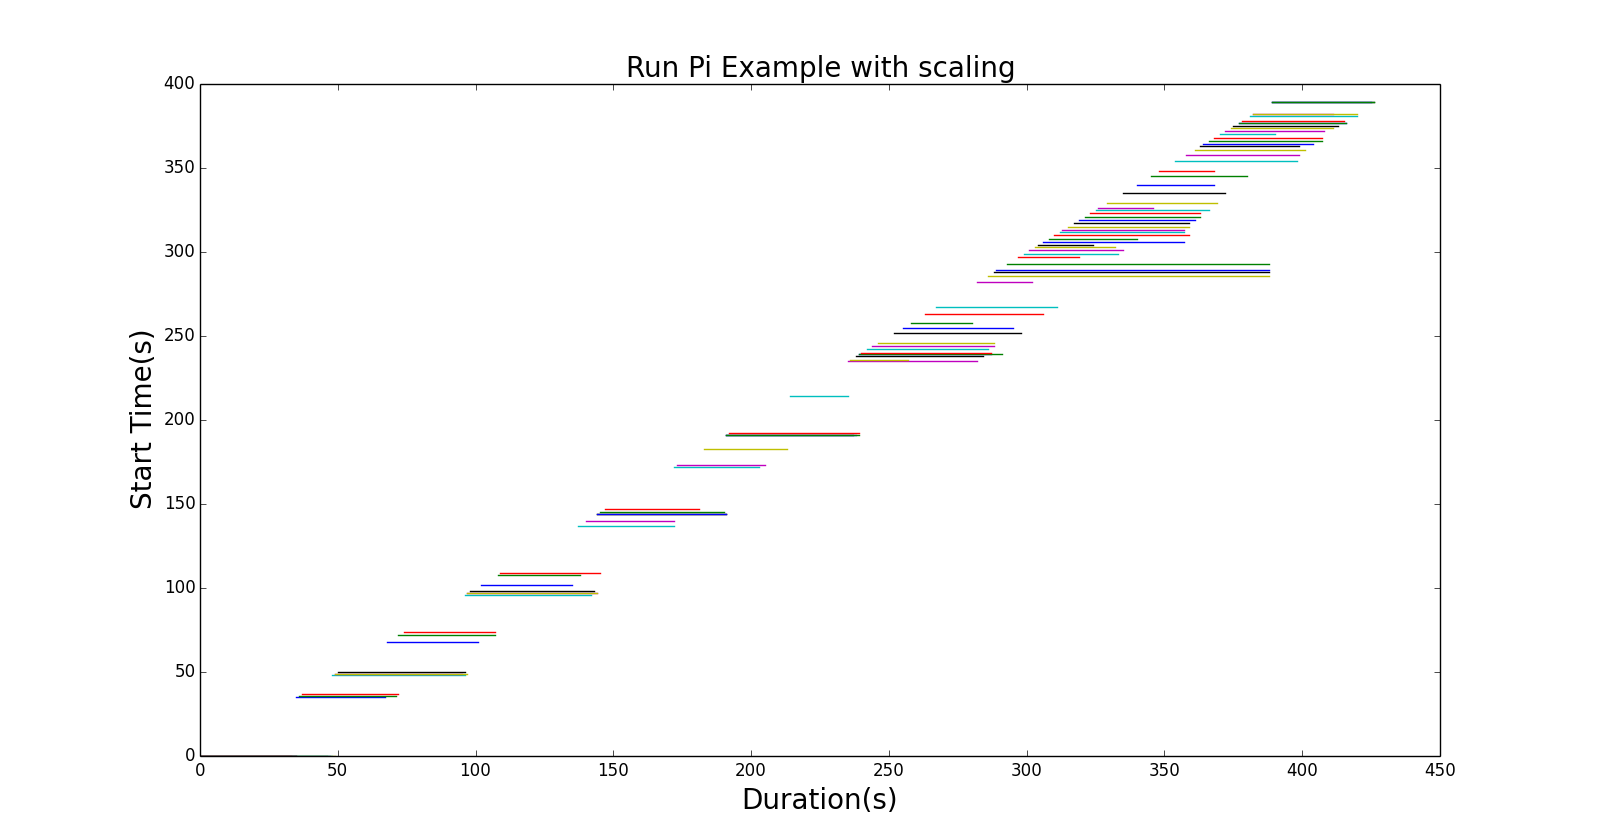
\includegraphics[width=0.9\textwidth,natwidth=1000,natheight=800]{scaling_pi.png}
 \caption{Pi Job with Auto-Scaling}
 \label{fig:scaling_pi}
 \end{figure}
\begin{figure}[ht!]
 \centering
 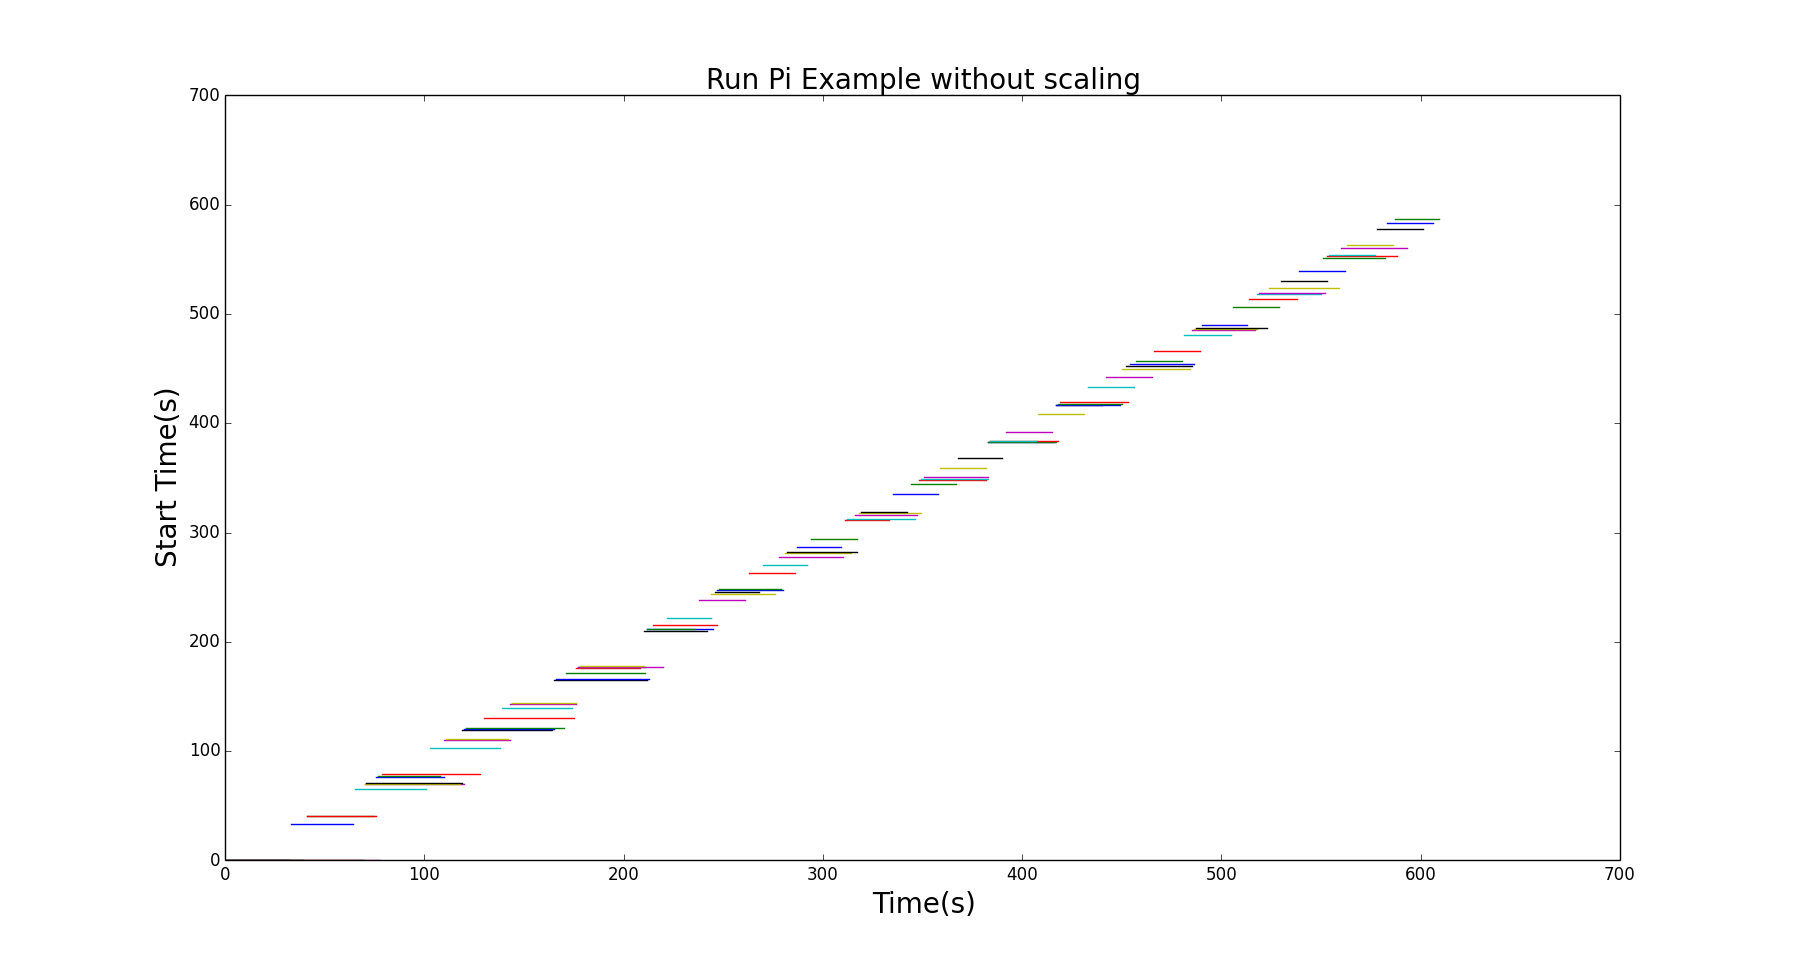
\includegraphics[width=0.9\textwidth,natwidth=1000,natheight=800]{no_scaling_pi.png}
 \caption{Pi Job without Auto-Scaling}
 \label{fig:no_scaling_pi}
 \end{figure}

\subsection{Running different jobs on auto scaling cluster}
We have run two different jobs on the same auto scaling cluster. The first job is (yarn jar hadoop-mapreduce-examples-2.7.1.2.3.2.0-2950.jar pi 100 10000000), and the second job is (yarn jar hadoop-mapreduce-examples-2.7.1.2.3.2.0-2950.jar pi 100 1000000000). Then we monitor the memory and CPU usage of two jobs from cluster, and the results are shown in \textbf{Figure~\ref{fig:memoryUtilization}} and \textbf{Figure~\ref{fig:cpuUtilization}}
\begin{figure}[ht!]
 \centering
 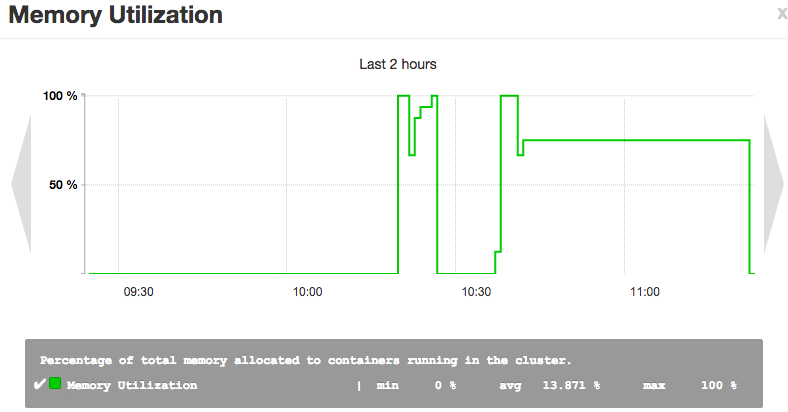
\includegraphics[width=0.8\textwidth,natwidth=1000,natheight=800]{memoryUtilization.png}
 \caption{Memory Utilization}
 \label{fig:memoryUtilization}
 \end{figure}
 
 \begin{figure}[ht!]
 \centering
 \includegraphics[width=0.8\textwidth,natwidth=1000,natheight=800]{cpuUtilization.png}
 \caption{CPU Utilization}
 \label{fig:cpuUtilization}
 \end{figure}
 
From \textbf{Figure~\ref{fig:memoryUtilization}}. We can see the duration time of memory usage of two jobs. The first bar's duration time is smaller than the second one because the first job is smaller than the second one. In the first bar, when the memory usage is approximately 100\%, our application will start the scale out process. After adding new instances into the cluster, the total memory of the cluster will increase, so the memory usage of the cluster will decrease. If there are more available memory, the Resource Manager will allocate free resources to pending jobs. After allocating, the total memory usage will increase too. When all jobs are finished, the memory usage will decrease to zero.
 
\section{Related Work}
In deployment, we used Go programming language library for AWS and consul, a tool for discovering and configuring services in our infrastructure. In monitoring, our application integrates Hadoop provisioning and monitoring capabilities with the Ambari(an open-source, cluster-management tool ) and ELK stack(combine three open source projects Elasticsearch, Logstash, and Kibana). For scaling, although Hadoop cluster is widely used nowadays, many researchers[3,4] challenge the viewpoint that scaling out using a cluster of commodity machines is better to run data analytic workloads. Rowstron[3] argues that single big memory servers may simply be more efficient than clusters, which can substantially change price points and complexity.  Appuswamy[4] evaluates scaling up versus scaling out across a range of analytic workloads and using four metrics: performance, cost, energy, and server density. In the last part of our project, we want to do similar studies in scaling out. It is interesting and useful to conduct research in determining when and how to scale out the cluster.


\section{Conclusion}
In conclusion, we have done much work in the deployment, monitoring and auto scaling of Hadoop Yarn Cluster. For deployment, we developed CLI to manage a cluster, provisioned a Hadoop cluster and managed Hadoop Service using Ambari. For monitoring, we employed Ambari metrics system for metrics collection. For auto scaling, we designed alert-based system to scale out/down, utilized scaling strategy by user defined policy and Ambari alert service, and implemented web UI to register cluster. During the configuration of the Elasticsearch, Logstash and Kibana, we have learned some basic knowledge about how the monitor and logging infrastructure works. Furthermore,  combining Logstash forwarder and Ambari logs will give us the opportunity to generate statically real-time logs for us to auto analyze and work out a more efficient scaling model. During the implementation of auto scaling, we tried different methods to determine when and how to scale out the YARN cluster. In the future, there are two improvements for our experiments. One is to run different kinds of testing jobs in Hadoop cluster. The other is to analyze the relationship between scaling out and various metrics like Hadoop Yarn memory usage and CPU usage.


% Generate the bibliography.
\begin{thebibliography}{4}


\bibitem{Wadkar}
Wadkar, Sameer, and Madhu Siddalingaiah
\newblock Monitoring Hadoop.
\newblock  Pro Apache Hadoop. Apress, 2014. 203-215.
\label{ref:wadkar}

\bibitem{EC2}
http://docs.aws.amazon.com/AWSEC2/latest/CommandLineReference/ec2-cli-launch-instance.html

\bibitem{Rowstron}
Rowstron, Antony, et al.
\newblock Nobody ever got fired for using Hadoop on a cluster.
\newblock  Proceedings of the 1st International Workshop on Hot Topics in Cloud Data Processing. ACM, 2012.

\bibitem{Appuswamy}
Appuswamy, Raja, et al.
\newblock Scale-up vs Scale-out for Hadoop: Time to rethink?
\newblock Proceedings of the 4th annual Symposium on Cloud Computing. ACM, 2013.
\bibitem{Ambari API}
\label{ref:ambariAPI}
Ambari API Reference Document 
\newblock https://github.com/apache/ambari/blob/trunk/ambari-server/docs/api/v1/index.md


\end{thebibliography}

\section{Appendix}



\begin{enumerate}

\item Add cluster demo ( https://goo.gl/SWiUsd )
\item Scaling up demo ( https://goo.gl/oIHwCu )
\item Scaling down demo ( https://goo.gl/QkBSWq )

\item Database schema for Instance pool
\begin{lstlisting}
CREATE TABLE `Ambari` (
  `id` bigint(20) NOT NULL AUTO_INCREMENT,
  `ambari_host` varchar(255) DEFAULT NULL,
  `ambari_pass` varchar(255) DEFAULT NULL,
  `ambari_port` varchar(255) DEFAULT NULL,
  `ambari_user` varchar(255) DEFAULT NULL,
  PRIMARY KEY (`id`)
) ENGINE=InnoDB AUTO_INCREMENT=2 DEFAULT CHARSET=latin1 
CREATE TABLE `cluster` (
  `id` bigint(20) NOT NULL AUTO_INCREMENT,
  `latest_scaling_activity` bigint(20) DEFAULT NULL,
  `operation_interval` int(11) DEFAULT NULL,
  `state` varchar(255) DEFAULT NULL,
  `ambari_id` bigint(20) DEFAULT NULL,
  PRIMARY KEY (`id`),
  KEY `FK_tq6aoyelc0pf02o5vy6d5qi5p` (`ambari_id`),
  CONSTRAINT `FK_tq6aoyelc0pf02o5vy6d5qi5p` FOREIGN KEY (`ambari_id`) REFERENCES `Ambari` (`id`)
) ENGINE=InnoDB AUTO_INCREMENT=2 DEFAULT CHARSET=latin1 
CREATE TABLE `metrics_alert` (
  `id` bigint(20) NOT NULL AUTO_INCREMENT,
  `alert_state` int(11) DEFAULT NULL,
  `definition_name` varchar(255) DEFAULT NULL,
  `name` varchar(255) DEFAULT NULL,
  `scaling_policy` int(11) DEFAULT NULL,
  `time_definition` int(11) DEFAULT NULL,
  `cluster_id` bigint(20) DEFAULT NULL,
  PRIMARY KEY (`id`),
  KEY `FK_qvgna8o8ug3nlp5n120llbgo` (`cluster_id`),
  CONSTRAINT `FK_qvgna8o8ug3nlp5n120llbgo` FOREIGN KEY (`cluster_id`) REFERENCES `Cluster` (`id`)
) ENGINE=InnoDB AUTO_INCREMENT=2 DEFAULT CHARSET=latin1 
CREATE TABLE `instance` (
  `id` bigint(20) NOT NULL AUTO_INCREMENT,
  `privateIP` varchar(255) DEFAULT NULL,
  `state` int(11) DEFAULT NULL,
  `cluster_id` bigint(20) DEFAULT NULL,
  PRIMARY KEY (`id`),
  KEY `FK_5nbl03hh8cth66xf8obiiguc` (`cluster_id`),
  CONSTRAINT `FK_5nbl03hh8cth66xf8obiiguc` FOREIGN KEY (`cluster_id`) REFERENCES `Cluster` (`id`)
) ENGINE=InnoDB DEFAULT CHARSET=latin1
\end{lstlisting}

\end{enumerate}
\end{document}
